\documentclass[compress]{beamer}
\usepackage{ifthen,verbatim}

\newcommand{\isnote}{}
\xdefinecolor{lightyellow}{rgb}{1.,1.,0.25}
\xdefinecolor{darkblue}{rgb}{0.1,0.1,0.7}

%% Uncomment this to get annotations
%% \def\notes{\addtocounter{page}{-1}
%%            \renewcommand{\isnote}{*}
%% 	   \beamertemplateshadingbackground{lightyellow}{white}
%%            \begin{frame}
%%            \frametitle{Notes for the previous page (page \insertpagenumber)}
%%            \itemize}
%% \def\endnotes{\enditemize
%% 	      \end{frame}
%%               \beamertemplateshadingbackground{white}{white}
%%               \renewcommand{\isnote}{}}

%% Uncomment this to not get annotations
\def\notes{\comment}
\def\endnotes{\endcomment}

\setbeamertemplate{navigation symbols}{}
\setbeamertemplate{headline}{\mbox{ } \hfill
\begin{minipage}{5.5 cm}
\vspace{-0.75 cm} \small
\end{minipage} \hfill
\begin{minipage}{4.5 cm}
\vspace{-0.75 cm} \small
\begin{flushright}
\ifthenelse{\equal{\insertpagenumber}{1}}{}{\hspace{0.2 cm} \insertpagenumber\isnote/\pageref{numpages}}
\end{flushright}
\end{minipage}\mbox{\hspace{0.2 cm}}\includegraphics[height=1 cm]{../cmslogo} \hspace{0.01 cm} \vspace{-1.05 cm}}

\newcommand{\s}[1]{{\mbox{\scriptsize #1}}}

\begin{document}
\begin{frame}
\vfill
\begin{center}
\textcolor{darkblue}{\Large Proposed Muon Alignment Constants}

\vfill
\begin{columns}
\column{0.4\linewidth}
\begin{center}
\large
Muon Alignment Group
\end{center}
\end{columns}

\vfill
 6 August, 2010

\end{center}
\end{frame}

%% \begin{notes}
%% \item This is the annotated version of my talk.
%% \item If you want the version that I am presenting, download the one
%% labeled ``slides'' on Indico (or just ignore these yellow pages).
%% \item The annotated version is provided for extra detail and a written
%% record of comments that I intend to make orally.
%% \item Yellow notes refer to the content on the {\it previous} page.
%% \item All other slides are identical for the two versions.
%% \end{notes}

\small

%% \begin{frame}
%% \frametitle{Outline}
%% \begin{itemize}\setlength{\itemsep}{0.75 cm}
%% \item 
%% \end{itemize}
%% %% \hspace{-0.83 cm} \textcolor{darkblue}{\Large Outline2}
%% \end{frame}

%% \section*{First section}
%% \begin{frame}
%% \begin{center}
%% \Huge \textcolor{blue}{First section}
%% \end{center}
%% \end{frame}

\begin{frame}
\frametitle{Outline}
\begin{itemize}
\item Not a polished version of the Muon DPG talk for Monday!
\item Just a list of what we plan to show (our internal sign-off)
\end{itemize}

\vfill
\hspace{-0.83 cm} \textcolor{darkblue}{\Large Basic statement}

\begin{itemize}
\item Proposing DT hardware alignment (what was signed-off May~12)
\begin{itemize}
\item there are systematic discrepancies between track-based (TB) and hardware (HW) geometries
\item we do not have a compelling argument that either is more correct or trustworthy than the other
\item we therefore provide the HW$-$TB difference as a systematic uncertainty
\end{itemize}
\item Proposing CSC track-based alignment plus HW for $\phi_x$ and $Z$ (what was signed-off May~19 with some $Z$ updates from HW)
\begin{itemize}
\item HW$-$TB comparisons are not at the same level as in the barrel
\item but TB$-$PG (photogrammetry) are $\sim$0.6~mm
\end{itemize}
\item Proposing Sasha's global position for all systems (good
agreement between Sasha's method, TB, and HW)
\end{itemize}
\end{frame}

\begin{frame}
\frametitle{HW$-$TB barrel comparison}
\begin{itemize}
\item First: it's important to emphasize that TB and HW agree with each other much better than either does with ideal geometry
\item Two independent techniques have ``found'' the muon chambers
\item Now we're working on the 4~mm-scale differences\ldots
\end{itemize}

\vfill
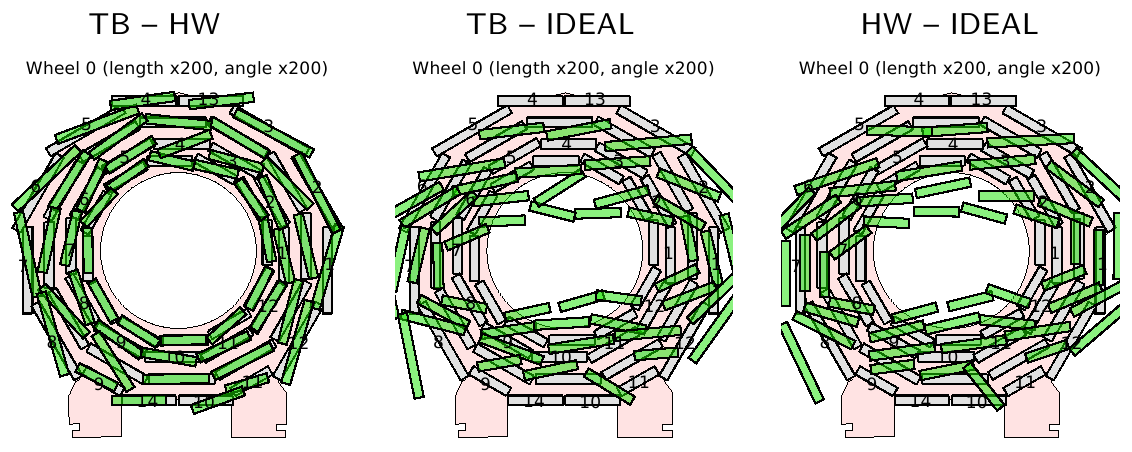
\includegraphics[width=\linewidth]{tb-hw_wheel0.png}

\mbox{\scriptsize {\bf N.B.} in this picture, displacements and angle differences have been exaggerated by 200$\times$\hspace{-1 cm}}
\end{frame}

\begin{frame}
\frametitle{HW$-$TB comparison}
\begin{columns}
\column{0.45\linewidth}
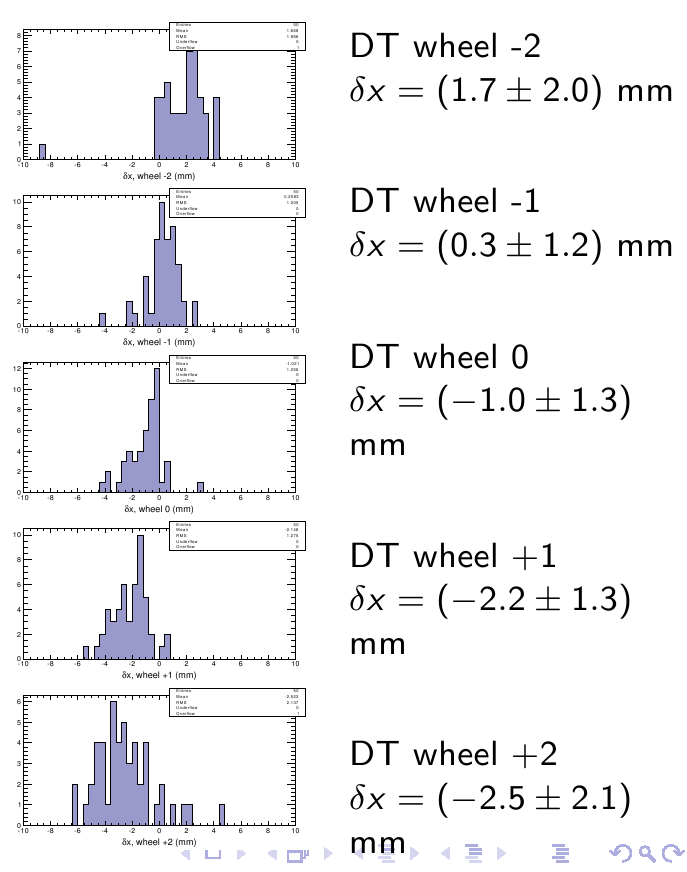
\includegraphics[width=\linewidth]{twist1.png}

\column{0.65\linewidth}
\begin{itemize}
\item Primary differences:
\begin{itemize}\setlength{\itemsep}{0.1 cm}
\item 5-chamber groups from wheel $-$2 \\ to wheel $+$2 seem to be coherently rotated: about 4~mm end-to-end
\item barrel compressed in $z$ by about 4~mm end-to-end
\item $\mathcal{O}(1.3\mbox{ mm})$ individual-chamber variations after that
\end{itemize}
\item<2> Same for all stations
\end{itemize}

\vfill

\only<1>{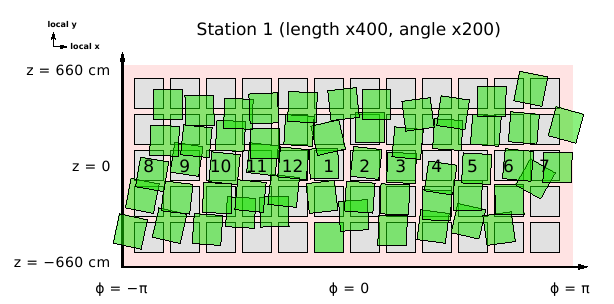
\includegraphics[width=\linewidth]{twist3_station1.png}}
\only<2>{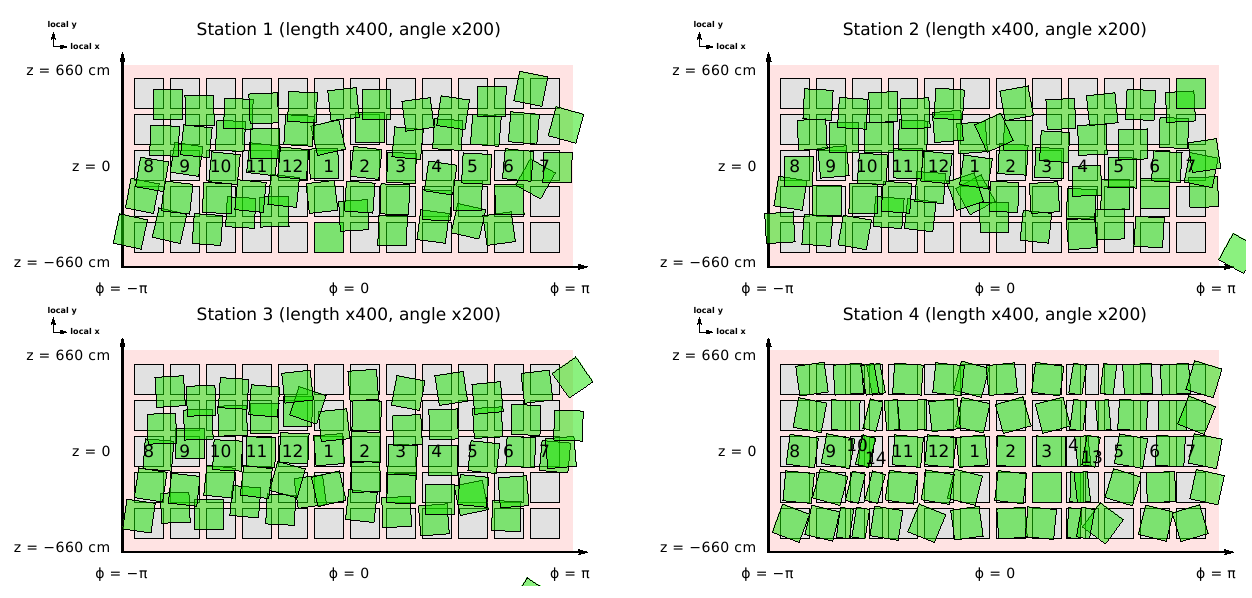
\includegraphics[width=\linewidth]{twist3.png}}
\end{columns}
\end{frame}

\begin{frame}
\frametitle{HW$-$TB comparison}
\begin{itemize}
\item Also seen at the level of residuals: these are $r\phi$ residuals
vs.\ $z$ in each 5-chamber group; dashed lines are boundaries \mbox{between chambers\hspace{-1 cm}}
\item Smooth transitions between chambers could be due to a coherent rotation in HW or a tracking bias in TB
\end{itemize}
\begin{center}
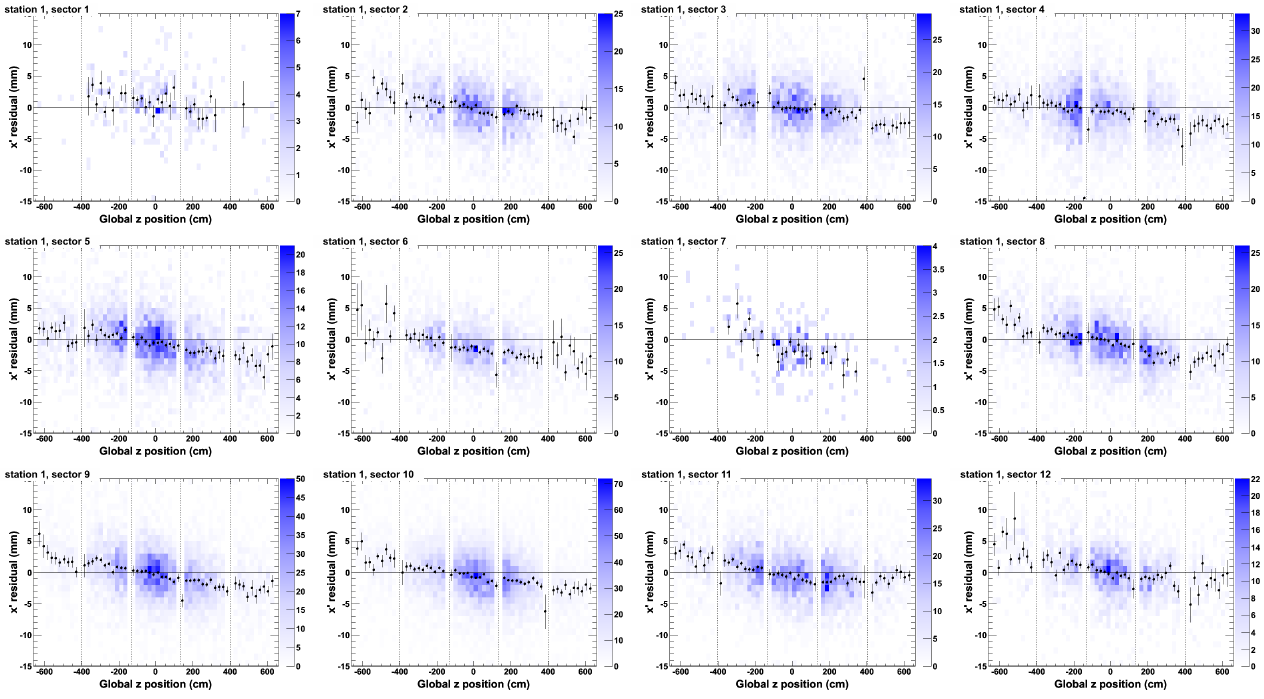
\includegraphics[width=0.9\linewidth]{twist2.png}
\end{center}

\vspace{-0.5 cm}
\mbox{\scriptsize {\bf N.B.} Vertical scales are $\pm$15~mm \hspace{-1 cm}}
\end{frame}

\begin{frame}
\frametitle{Station-by-station dependence}
\begin{columns}
\column{0.5\linewidth}
\begin{itemize}
\item If the effect were due to a bias in input tracks, e.g.\ a global
distortion of the tracker leading to $z$-dependent $\Delta \phi$
errors, then its magnitude would scale from distance from the tracker

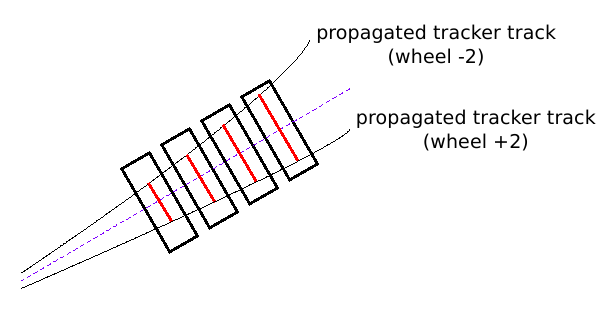
\includegraphics[width=\linewidth]{growth_with_station.png}

\item Test: fit each 5-chamber group of residuals to a straight line
(50 in all) and make histograms of the resulting slopes
\item Result: strongly peaked at the same slope in all four stations
\end{itemize}

\column{0.5\linewidth}
\begin{columns}
\column{0.5\linewidth}
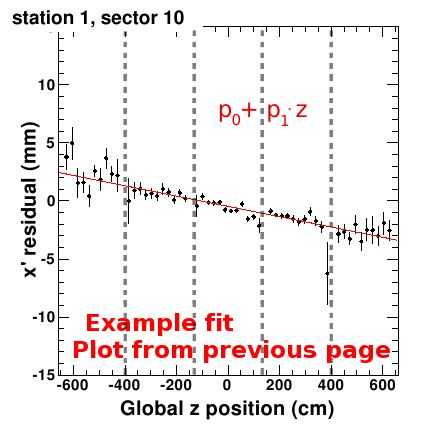
\includegraphics[width=\linewidth]{growth_with_station2.png}
\column{0.5\linewidth}
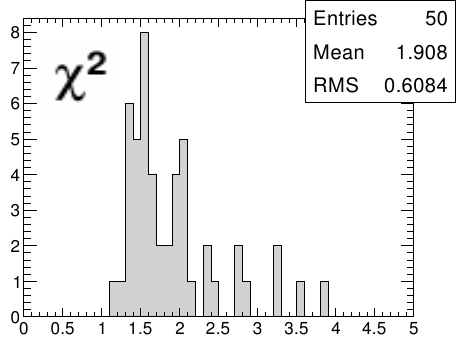
\includegraphics[width=\linewidth]{growth_with_station_chi2.png}
\end{columns}

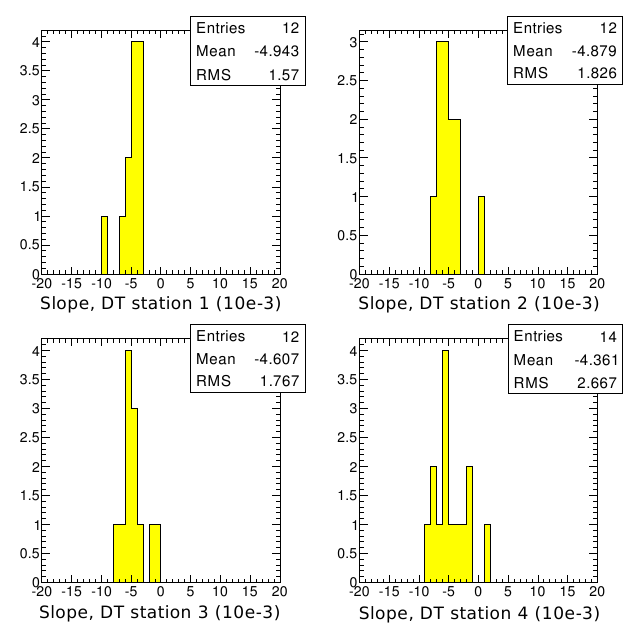
\includegraphics[width=\linewidth]{growth_with_station3.png}
\end{columns}
\end{frame}

\begin{frame}
\frametitle{0~T PG$-$HW test}
\begin{itemize}
\item If the trend were a weak mode of the HW alignment procedure, it
would be present in 0~T data as well
\item Photogrammetry (PG) data are available for 0~T, with
\textcolor{red}{x~mm} for inside-of-wheel resolutions and \textcolor{red}{y~mm} for
between-wheel resolutions
\item No evidence of 4~mm systematic trend from wheel $-$2 to wheel $+$2
\end{itemize}

\vfill
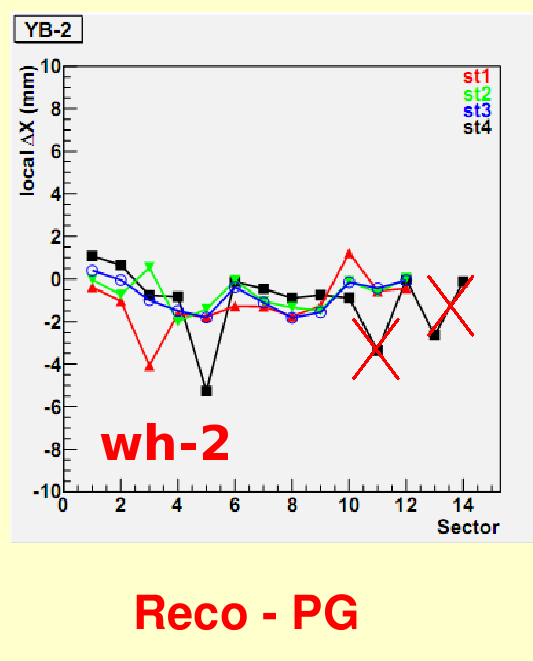
\includegraphics[width=0.19\linewidth]{hw_0T_vsPG_m2.png}
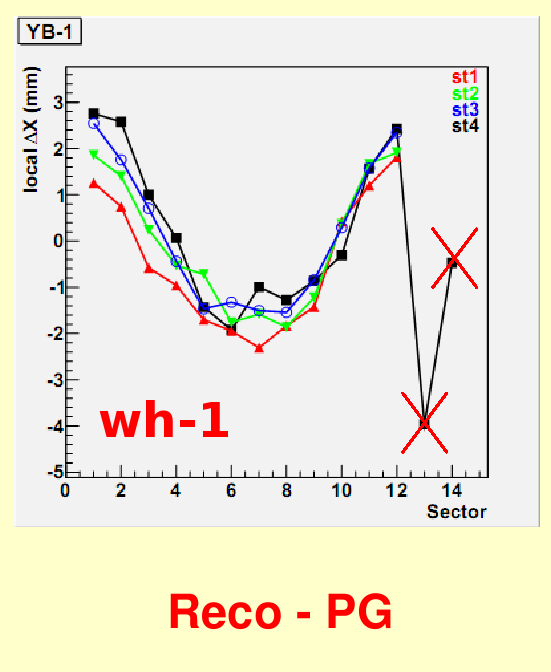
\includegraphics[width=0.19\linewidth]{hw_0T_vsPG_m1.png}
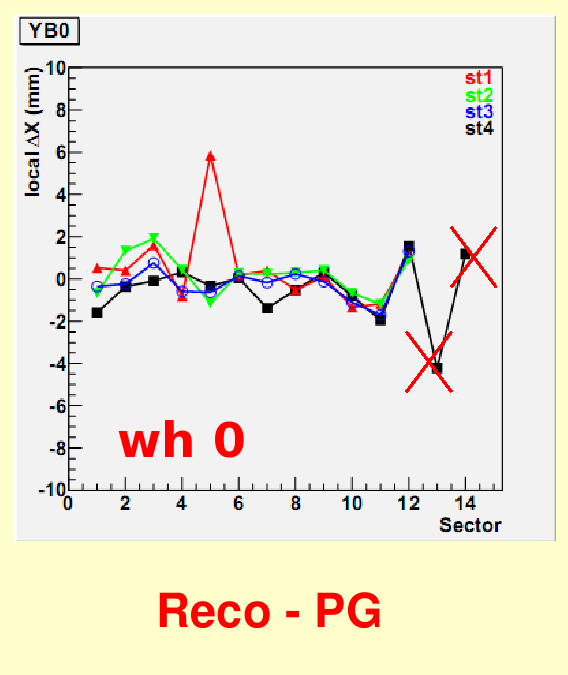
\includegraphics[width=0.19\linewidth]{hw_0T_vsPG_ze.png}
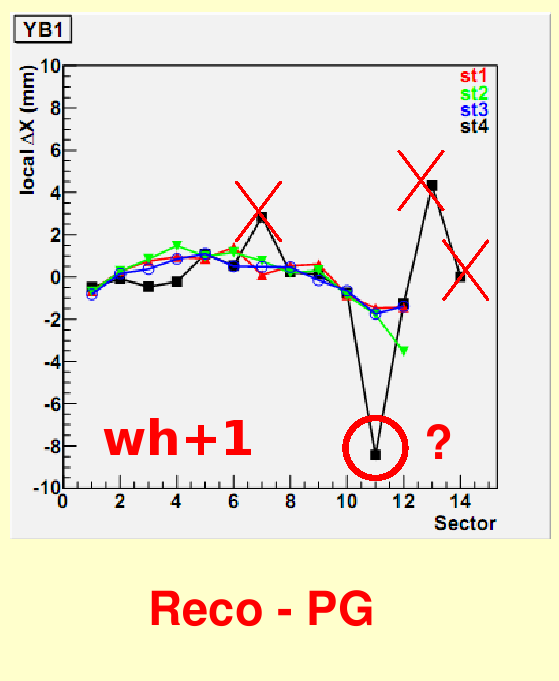
\includegraphics[width=0.19\linewidth]{hw_0T_vsPG_p1.png}
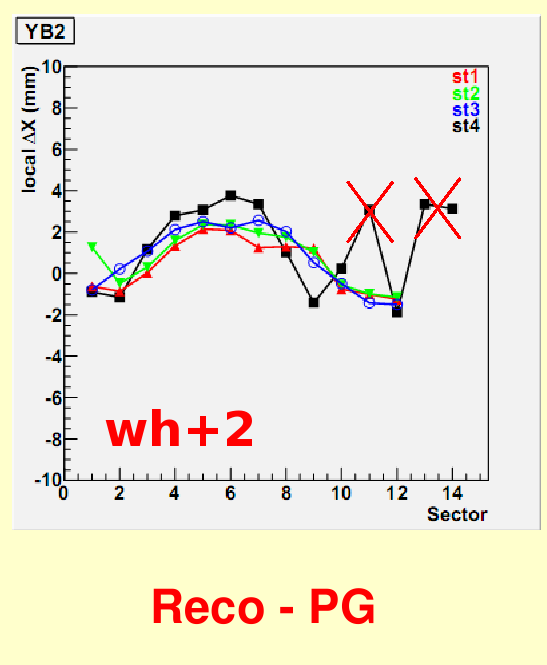
\includegraphics[width=0.19\linewidth]{hw_0T_vsPG_p2.png}

\mbox{\scriptsize {\bf N.B.} Vertical scales are $\pm$10~mm except wheel $-$1, which is $-$5 to 3~mm. \hspace{-1 cm}}
\end{frame}

\begin{frame}
\frametitle{Tiltmeter test}

\vspace{0.25 cm}
\begin{columns}
\column{0.35\linewidth}
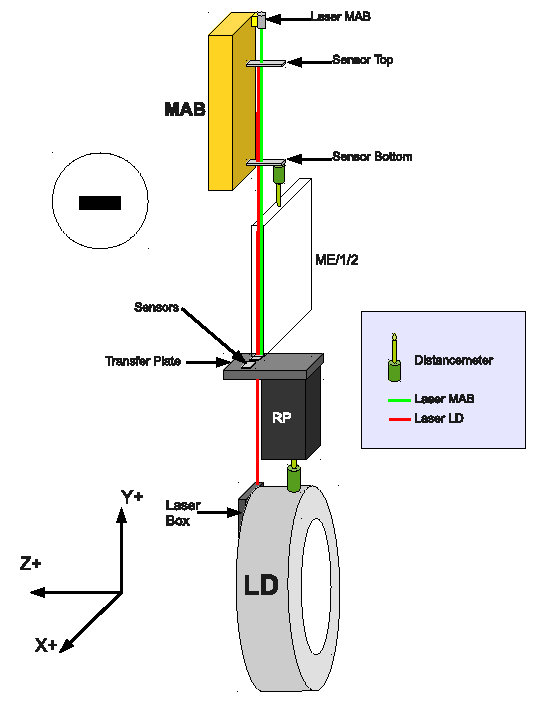
\includegraphics[width=\linewidth]{link_hardware_diagram2.png}

\column{0.75\linewidth}
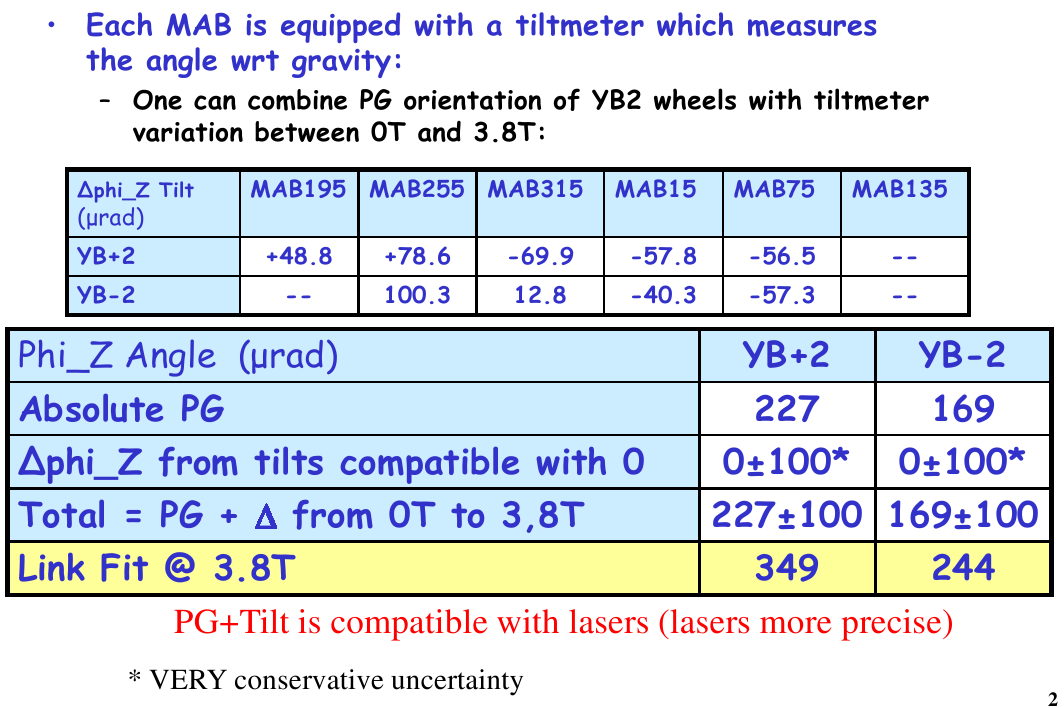
\includegraphics[width=\linewidth]{inclinometers.png}
\end{columns}

\vfill
\begin{itemize}
\item Link system between barrel and endcap connects to end of barrel hardware alignment devices (MAB) 4.5~m from the beamline
\item Constraint from gravity direction $+$ PG: \mbox{110 $\pm$ 140~$\mu$rad} $\to$ \mbox{0.47 $\pm$ 0.63~mm} at barrel ends, in contraction with TB's 4~mm
\item Independent of barrel alignment \textcolor{red}{\scriptsize (Does it assume that the MABs are rigid and ideal?  I still don't understand the comment in HyperNews)}
\end{itemize}
\end{frame}

\begin{frame}
\frametitle{Endcap alignment}

\begin{columns}
\column{0.5\linewidth}
\begin{itemize}
\item Several different sources of information:
\begin{itemize}
\item tilting ($\phi_x$) and motion toward magnet: straight line monitors (HW)
\item chambers-within-disks ($r\phi$, $\phi_z$): beam-halo tracks and
PG, weighted to prefer tracks where available
\item disks-relative-to-tracker (global $x$, $y$, $\phi_z$): cosmic
$p_T > 100$~GeV/$c$ tracks\textcolor{red}{$^*$}
\item final $z$ positions: transfer lines (HW)
\end{itemize}
\item All are unaffected by RPC-bias or GPR-removal bugs, except \textcolor{red}{$^*$},
which was re-run: see browser
\end{itemize}

\column{0.45\linewidth}
Beam-halo vs.\ PG:

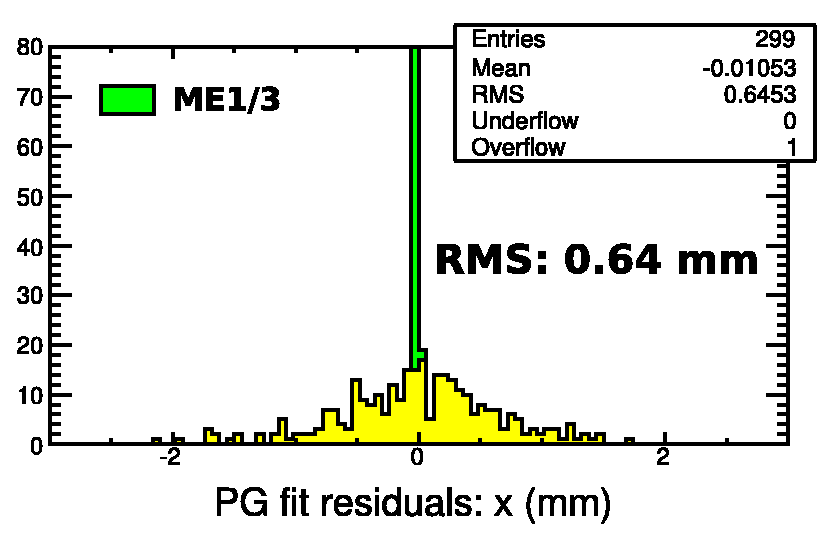
\includegraphics[width=\linewidth]{beamhalo-PG.png}

Disk position from cosmic GlobalMuons (\only<1>{before alignment}\only<2>{after alignment}):

\only<1>{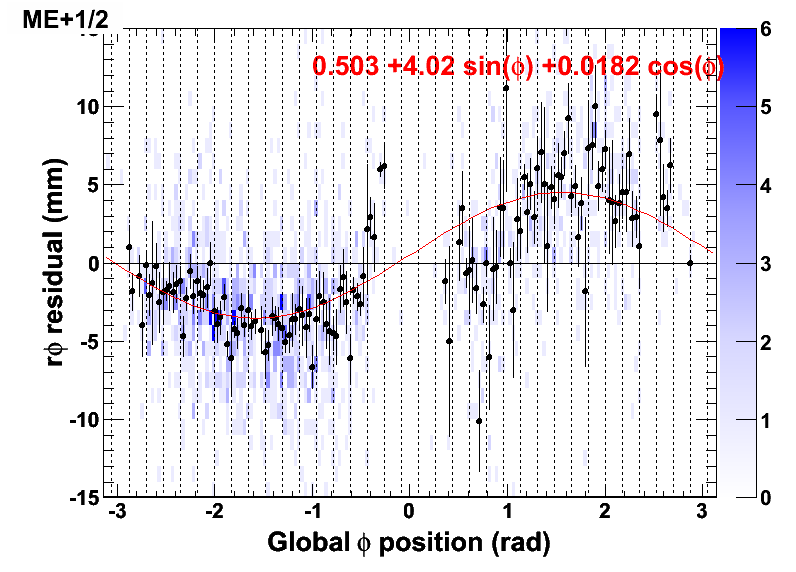
\includegraphics[width=\linewidth]{map_CSCvsphi_x_before.png}}
\only<2>{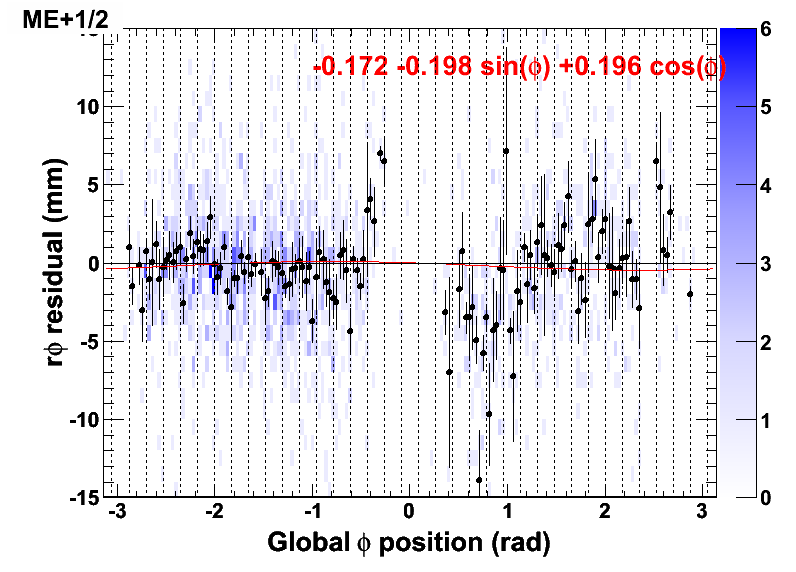
\includegraphics[width=\linewidth]{map_CSCvsphi_x_after.png}}
\end{columns}
\end{frame}

\begin{frame}
\frametitle{Endcap $z$ positions}
\begin{itemize}
\item Still need to be applied
\item Is this the latest distribution?  Why does it have this pattern?
\item Shouldn't it be approximately
\begin{itemize}
\item 14~mm for ME1/1 (inward)
\item 7~mm for all other stations (same global direction)
\end{itemize}
\end{itemize}

\begin{center}
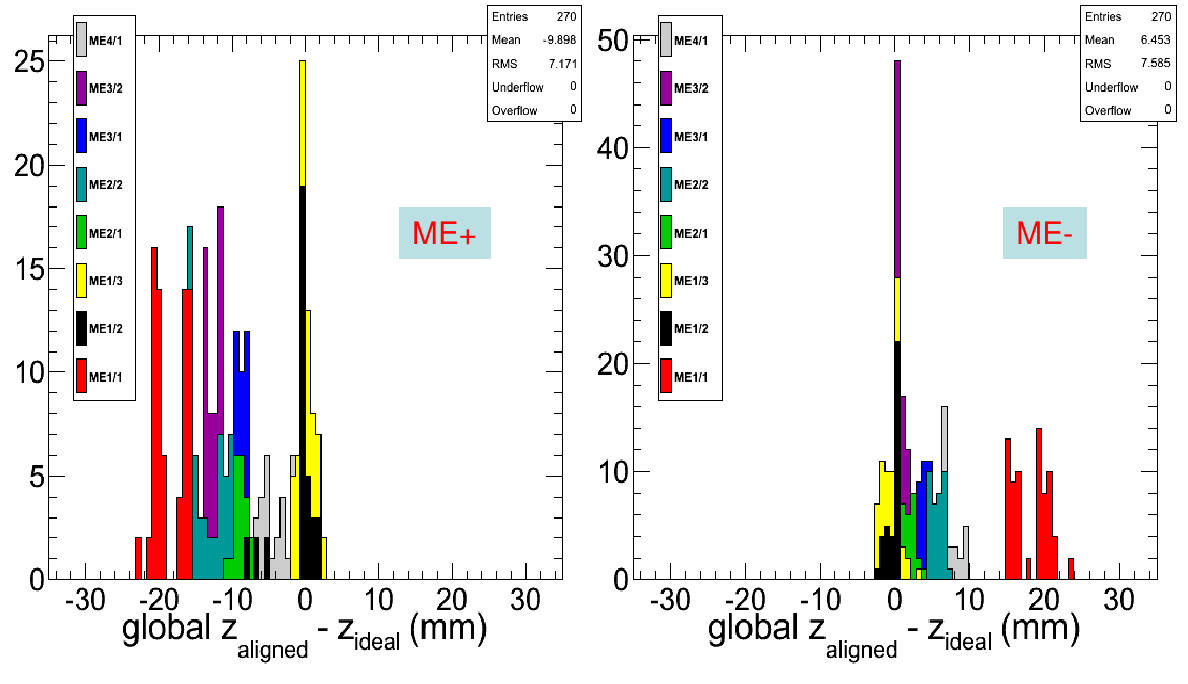
\includegraphics[width=0.9\linewidth]{endcap_z-split_1.png}
\end{center}
\end{frame}

\begin{frame}
\frametitle{Locations of constants}
\begin{itemize}
\item DT HW alignment: ?
\item CSC HW $\phi_x$ $+$ beam-halo $+$ cosmics-disk:

{\tt \scriptsize /afs/cern.ch/user/p/pivarski/public/JUN5\_CSC\_beamhalo-PG-diskXYphiZ.db}

Updated cosmics-disk plots in browser: \href{http://hepr8.physics.tamu.edu/mual/browser/}{\tt \scriptsize \textcolor{blue}{http://hepr8.physics.tamu.edu/mual/browser/}} ``ring\_data\_gprsasha''


\item CSC HW $\phi_x$ $+$ beam-halo $+$ cosmics-disk $+$ HW $Z$: needs to be created from the above $+$ the latest HW SQLite file

\item Sasha's GlobalPositionRcd: ?
\end{itemize}
\label{numpages}
\end{frame}

\end{document}
